%%%%%%%%%%%%%%%%%%%%%%%%%%%%%%%%%%%%%%%%%%%%%%%%%%%%%%%%%%%%%%%%%%%%%%%%%%%%%%%%%%%%%%%
%%%%%%%%%%%%%%%%%%%%%%%%%%%%%%%%%%%%%%%%%%%%%%%%%%%%%%%%%%%%%%%%%%%%%%%%%%%%%%%%%%%%%%%
% 
% This top part of the document is called the 'preamble'.  Modify it with caution!
%
% The real document starts below where it says 'The main document starts here'.

\documentclass[12pt]{article}

\usepackage{amssymb,amsmath,amsthm}
\usepackage[top=1in, bottom=1in, left=1.25in, right=1.25in]{geometry}
\usepackage{fancyhdr}
\usepackage{graphicx}
\usepackage{enumerate}
\usepackage{verbatim}
\usepackage{listings}
\usepackage{float}



% Comment the following line to use TeX's default font of Computer Modern.
\usepackage{times,txfonts}

\newtheoremstyle{homework}% name of the style to be used
  {18pt}% measure of space to leave above the theorem. E.g.: 3pt
  {12pt}% measure of space to leave below the theorem. E.g.: 3pt
  {}% name of font to use in the body of the theorem
  {}% measure of space to indent
  {\bfseries}% name of head font
  {:}% punctuation between head and body
  {2ex}% space after theorem head; " " = normal interword space
  {}% Manually specify head
\theoremstyle{homework} 

% Set up an Exercise environment and a Solution label.
\newtheorem*{exercisecore}{\@currentlabel}
\newenvironment{exercise}[1]
{\def\@currentlabel{#1}\exercisecore}
{\endexercisecore}

\newcommand{\localhead}[1]{\par\smallskip\noindent\textbf{#1}\nobreak\\}%
\newcommand\solution{\localhead{Solution:}}



% \newcommand{includematlab}[1]{\verbatiminput{#1}}

%%%%%%%%%%%%%%%%%%%%%%%%%%%%%%%%%%%%%%%%%%%%%%%%%%%%%%%%%%%%%%%%%%%%%%%%
%
% Stuff for getting the name/document date/title across the header
\makeatletter
\RequirePackage{fancyhdr}
\pagestyle{fancy}
\fancyfoot[C]{\ifnum \value{page} > 1\relax\thepage\fi}
\fancyhead[L]{\ifx\@doclabel\@empty\else\@doclabel\fi}
\fancyhead[C]{\ifx\@docdate\@empty\else\@docdate\fi}
\fancyhead[R]{\ifx\@docauthor\@empty\else\@docauthor\fi}
\headheight 15pt

\def\doclabel#1{\gdef\@doclabel{#1}}
\doclabel{Use {\tt\textbackslash doclabel\{MY LABEL\}}.}
\def\docdate#1{\gdef\@docdate{#1}}
\docdate{Use {\tt\textbackslash docdate\{MY DATE\}}.}
\def\docauthor#1{\gdef\@docauthor{#1}}
\docauthor{Use {\tt\textbackslash docauthor\{MY NAME\}}.}
\makeatother

%% General formatting parameters
\parindent 0pt
\parskip 12pt plus 1pt

% Shortcuts for blackboard bold number sets (reals, integers, etc.)
\newcommand{\Reals}{\ensuremath{\mathbb R}}
\newcommand{\Nats}{\ensuremath{\mathbb N}}
\newcommand{\Ints}{\ensuremath{\mathbb Z}}
\newcommand{\Rats}{\ensuremath{\mathbb Q}}
\newcommand{\Cplx}{\ensuremath{\mathbb C}}
%% Some equivalents that some people may prefer.
\let\RR\Reals
\let\NN\Nats
\let\II\Ints
\let\CC\Cplx

%%%%%%%%%%%%%%%%%%%%%%%%%%%%%%%%%%%%%%%%%%%%%%%%%%%%%%%%%%%%%%%%%%%%%%%%%%%%%%%%%%%%%%%
%%%%%%%%%%%%%%%%%%%%%%%%%%%%%%%%%%%%%%%%%%%%%%%%%%%%%%%%%%%%%%%%%%%%%%%%%%%%%%%%%%%%%%%
% 
% The main document start here.

% The following commands set up the material that appears in the header.
\doclabel{Math 426: Homework 3}
\docauthor{Stefano Fochesatto}
\docdate{September 16, 2020}

\newcommand{\vv}{\mathbf{v}}
\begin{document}





\begin{exercise}{DM 1}
Write down the $4^{\rm th}$ order Taylor
polynomial of $\sqrt{x}$ centered at $x=1$.  Let
$P(x)$ denote this polynomial. If $1\le x \le 2$,
what can you say about the size of $|\sqrt{x}-P(x)|$?
Hint: Use the remainder term!
\end{exercise} 

\solution
The forth order taylor polynomial of $\sqrt{x}$ centered at $x = 1$, 
\begin{equation*}
  P(x) = 1 + \dfrac{1}{2}(x-1)  - \dfrac{1}{8}(x - 1)^2 + \dfrac{1}{16}(x - 1)^3 - \dfrac{5}{128}(x - 1)^4
\end{equation*}
From Taylor's Theorem we know that there exists some $\xi \in (1, x)$ such that,
\begin{equation*}
  \sqrt(x) = P(x) + \frac{7}{256}(\xi)^{-\dfrac{9}{2}}(x - 1)^5
\end{equation*}
Calculating the maximum error for $1\le x \le 2$,
\begin{align*}
  |\sqrt{x}-P(x)| &= \frac{7}{256}|(\xi)^{-\dfrac{9}{2}}|(x - 1)^5,\\
  &\leq \frac{7}{256}|1|(x - 1)^5,\\
  &\leq \frac{7}{256}|1|((2) - 1)^5,\\
  &\leq \frac{7}{256}.
\end{align*}
Note that the fifth derivative is largest on the interval $(1,x)$ when $\xi$ is closest to $1$ and the remaining expression is 
largest when $x = 2$. Thus giving us a maximum error of $\frac{7}{256}$.












\begin{exercise}{Chapter 4: 2 (b)}

For full credit you must write your own version of Newton's method.
Your function should have the signature

\begin{verbatim} 
function [r,hist] = hw3newton(f,fp,x1,ftol,xtol,Nmax)

end
\end{verbatim}

The input values are
\begin{itemize}
\item \texttt{f}, the function to find a root of.
\item \texttt{fp}, the derivative function of \texttt{f}.
\item \texttt{x1}, the first iteration value.
\item \texttt{ftol}, the tolerance for stopping based of the value of \texttt{f}
\item \texttt{xtol}, the tolerance for stopping based on changes in \texttt{x}
\item \texttt{Nmax}, the maximum number of iterations
\end{itemize}

Your function should exit with an error if more than \texttt{Nmax} iterations
are used.  It should return whenever $|f(x)|<f_{\text{tol}}$ or $|x_n-x_{n-1}|<x_{\text{tol}}$.

The return values should be \texttt{r}, the estimate of the root's position,
and \texttt{hist}, a list of all estimates starting with \texttt{x1} and ending with the final estimate \texttt{r}.

Test that your function works by finding three different ways to call it
so that iteration stops for each of the three possible reasons.

To answer the problem in the textbook, you will want to call your functin with 
$x_{\rm tol}=0$ to ensure that only the $f_{\rm tol}$ condition is used
to stop the iteration.\\

\textbf{Code:}
\lstinputlisting{hw3newton.m}


\solution
Testing our function works by demonstrating the 3 different ways it can terminate, \\

\textbf{Console:}
\lstinputlisting{newton}
Running our routine for the function with $x1 = 5$ and tolerance for $f(x)$ at $10^{-8}$,
\begin{equation*}
  f(x) = (5-x)e^x - 5.
\end{equation*}
\textbf{Console:}
\lstinputlisting{newton1}
Looking at the values for our error when compared to a more precise wolfram computation we can see clear quadratic convergence and to get to an $f(x)$ tolerance as small as $10^{-16}$ would only require one more step.
Furthermore we can show this by calculating, 
\begin{equation*}
  \lim_{k\to\infty} \dfrac{|e_{k+1}|}{|e_{k}|^2} \approx C.
\end{equation*} 
Where C is a constant, and luckily since our error converges so fast we can see that after the first iteration this limit will be approximately 1.\\

\textbf{Console:}
\lstinputlisting{newton2}







\end{exercise}











\begin{exercise}{Chapter 4: 6 (a,b)}
Also, use your \texttt{hw3newton} function from the previous problem
to compute the location of the minimum, and generate a plot that indicates that your computation succeeded. Consider the 
function, 
\begin{equation*}
  h(x) = \dfrac{x^4}{4} - 3x.
\end{equation*}
In this problem, we will see how to use Newton's method to find the minimum of the function $h(x)$.\\

\end{exercise}
\begin{enumerate}
  \item[\textbf{a.}] Derive a function f that has a root at the point where $h$ achieves it minimum. Write down the formula for Newton's
  method applied for $f$. \\

  \solution Recall that at the minima and maxima of continuous, differentiable function the slope is equal to zero, and thus let $f(x) = h'(x)$. Calculating the derivative
  we get, 
  \begin{equation*}
    f(x) = x^3 - 3
  \end{equation*}
  To find the roots of $f$ using Newton's method we also need to find $f'$,
  \begin{equation*}
    f'(x) = 3x^2.
  \end{equation*}
  Stating the iterative formula for Newton's method derived from the first order Taylor Polynomial,
  \begin{equation*}
    x_{k+1} = x_k - \dfrac{x_k^3 - 3}{3x_k^2}
  \end{equation*}
  \vspace{.25in}

  \item[\textbf{b.}]Take one step (by hand) with Newton's method starting with $x_0 = 1$.\\
 
  \solution Simply substituting $x_0 = 1$ into the previous formula,
  \begin{align*}
    x_1 &= 1 - \dfrac{1^3 - 3}{3(1)^2},\\
    &= 1 + \dfrac{2}{3},\\
    &=\dfrac{5}{3}.\\
  \end{align*}


\end{enumerate}


\begin{exercise}{Chapter 4: 7} In finding a root with Newton's method, an initial guess of $x_0 = 4$ with $f(x_0) = 1$ 
  leads to $x_1 = 3$. What is the derivative of $f$ at $x_0$\\
  
  \solution Simply substituting our given values to the iterative formula for Newton's method gives us,
  \begin{align*}
    x_{k+1} &= x_k - \dfrac{f(x_k)}{f'(x_k)},\\
    3 &= 4 - \dfrac{1}{f'(x_0)},\\
    -1 &=-\dfrac{1}{f'(x_0)},\\
    1 &= f'(x_0).
  \end{align*}

\end{exercise}

\begin{exercise}{Chapter 4: 10} Consider that the function,
  \begin{equation*}
    f(x) = \dfrac{x^2 - 2x + 1}{x^2 - x - 2}
  \end{equation*}
  has exactly one zero in the interval $[0,3]$, at $x = 1$. Using $a = 0$ and $b = 3$, run the bisection method on $f(x)$ with a 
  stopping tolerance of $\delta = 1e-3$. Explain why it does not appear to converge to the root. Why does the Intermediate Value Theorem
  $not$ guarantee that there is a root in $[0, 1.5]$ or in $[1.5,3]$\\
  
  Use MATLAB to plot this function over the interval in a way that makes it cleat what is going on. [Hint: You may want to use the plot command 
  over two different $x$ intervals separately in order to show the behavior properly.]\\
  
  \solution Consider the plot of the function,
  \begin{equation*}
    f(x) = \dfrac{x^2 - 2x + 1}{x^2 - x - 2}.
  \end{equation*}

  \begin{figure}[H]
    \caption{f(x) on the interval of $[0,3]$}
    \centering
    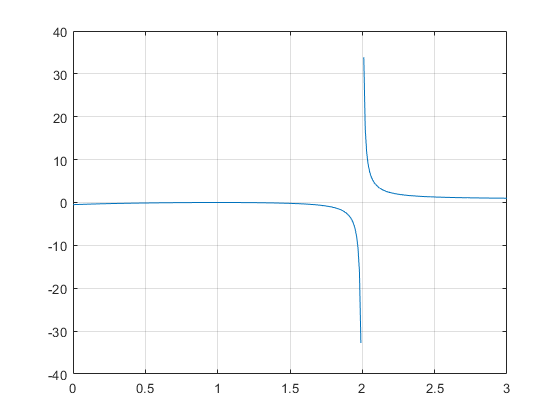
\includegraphics[width = .75 \textwidth,]{entire.png}
    \end{figure}
  Note that there is an infinite discontinuity at $x = 2$. Recall that the Intermediate Value Theorem states that,

If $f(x)$ is continuous on the interval $[a,b]$ and $y$ lies between $f(a)$ and $f(b)$, then there exists some point $x \in [a,b]$ where $f(x) = y$.
As a corollary we know that if $f(a)$ and $f(b)$ have opposite signs then $y = 0 \in [a,b]$ which is the principle behind bisection. Demonstrating why IMV Theorem 
fails to find a root of x = 1 on the interval $[0,1.5]$,
\begin{equation*}
  f(0) = \dfrac{0^2 - 2(0) + 1}{0^2 - 0 - 2} = -\dfrac{1}{2},
\end{equation*}
\begin{equation*}
  f(\frac{3}{2}) = \frac{(\frac{3}{2})^2 - 2(\frac{3}{2}) + 1}{(\frac{3}{2})^2 - \frac{3}{2} - 2} = -\frac{1}{5},
\end{equation*}\\
\begin{figure}[H]
  \caption{f(x) on the interval of $[0,1.5]$}
  \centering
  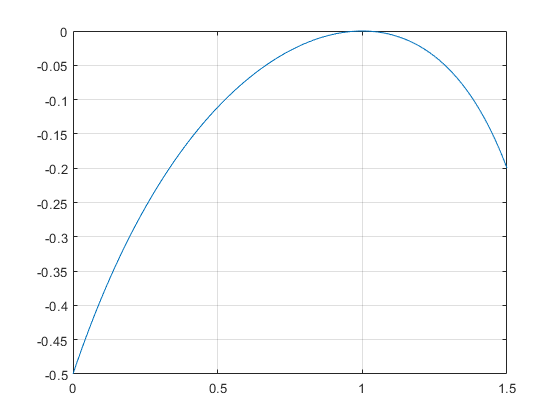
\includegraphics[width = .75 \textwidth,]{samesign.png}
  \end{figure}
Therefore we can see both bounds have the same sign and thus fails the corollary to IMV Theorem so bisection will not find root $x = 1$. \\
\vspace{1in}

Demonstrating why IMV Theorem fails to find a root of on the interval $[1.5,1]$, simply by demonstrating discontinuity at x = 2. Consider the following limit,
\begin{equation*}
  lim_{x \to 2} \dfrac{x^2 - 2x + 1}{x^2 - x - 2} = \dfrac{1}{0}.
\end{equation*}

\begin{figure}{H}
  \caption{f(x) on the interval of $[1.5,3]$}
  \centering
  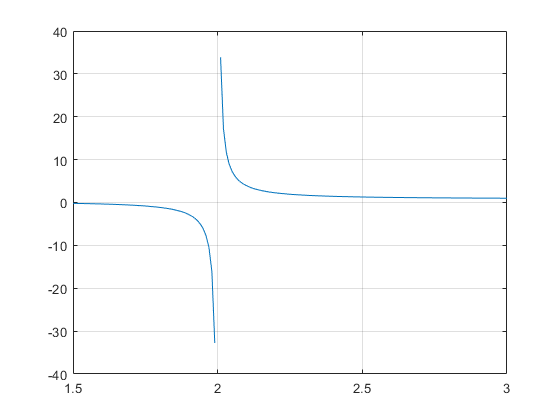
\includegraphics[width = .75 \textwidth,]{discon.png}
  \end{figure}

Thus we have shown that the limit of $f(x)$ where $x \to 2$ does not exists and therefore $f(x)$ is discountinuous on the interval $[1.5,1]$. Interestingly since the $f(2)$ is an infinite discontinuity
it seems to explain why our bisection algorithm converges to $x = 2$ as the limits on either side of $2$ have opposite signs.\\

\textbf{Console:}
\lstinputlisting{IMV}


\end{exercise}

\end{document}